%\title{emnlp 2017 instructions}
% File emnlp2017.tex
%

\documentclass[11pt,letterpaper]{article}
\usepackage{emnlp2017}
\usepackage{times}
\usepackage{latexsym}
\usepackage{hyperref}
\usepackage{graphicx}
\usepackage{minted}
\usepackage{mathtools}
\usepackage{subcaption}
\usepackage{caption}
\usepackage{xcolor}
\usepackage{multirow}
\usepackage{amssymb}
\usepackage{bm}
\usepackage{wrapfig}
%\usepackage[section]{placeins}
%\usepackage[draft]{hyperref}
% Uncomment this line for the final submission:
%\emnlpfinalcopy
%\newcommand{\vg}[1]{\textcolor{red}{\bf\small [#1 --VG]}}
%\newcommand{\hj}[1]{\textcolor{magenta}{\bf\small [#1 --HJ]}}
%  Enter the EMNLP Paper ID here:
\def\emnlppaperid{4}

% To expand the titlebox for more authors, uncomment
% below and set accordingly.
% \addtolength\titlebox{.5in}    

\newcommand\BibTeX{B{\sc ib}\TeX}


\title{Shakespearizing Modern Language Using Copy-Enriched Sequence-to-Sequence Models}

% Author information can be set in various styles:
% For several authors from the same institution:
% \author{Author 1 \and ... \and Author n \\
%         Address line \\ ... \\ Address line}
% if the names do not fit well on one line use
%         Author 1 \\ {\bf Author 2} \\ ... \\ {\bf Author n} \\
% For authors from different institutions:
% \author{Author 1 \\ Address line \\  ... \\ Address line
%         \And  ... \And
%         Author n \\ Address line \\ ... \\ Address line}
% To start a seperate ``row'' of authors use \AND, as in
% \author{Author 1 \\ Address line \\  ... \\ Address line
%         \AND
%         Author 2 \\ Address line \\ ... \\ Address line \And
%         Author 3 \\ Address line \\ ... \\ Address line}
% If the title and author information does not fit in the area allocated,
% place \setlength\titlebox{<new height>} right after
% at the top, where <new height> can be something larger than 2.25in
\author{Anonymous authors \\
  {\tt publication@emnlp2017.net}}

\date{}

\begin{document}

\maketitle

\begin{abstract}
Variations in writing styles are commonly used to adapt the content to a specific context, audience, or purpose. However, applying stylistic variations is still by and large a manual process, and there have been little efforts towards automating it. In this paper we explore automated methods to transform text from modern English to Shakespearean English using an end to end trainable neural model with pointers to enable copy action. To tackle limited amount of parallel data, we pre-train embeddings of words by leveraging external dictionaries mapping Shakespearean words to modern English words as well as additional text. Our methods are able to get a BLEU score of $31+$, an improvement of $\approx6$ points above the strongest baseline.

\end{abstract}

\section{Introduction}

%Motivation for style transfer

% Style. Prior works
Transforming style of text can be considered as application of lexical (e.g. using a synonym) and grammatical transformations (e.g. active vs passive voice). However, stylistic variations of a text, in contrast to machine translation, share significant amount of lexical and grammatical properties. 

% introduce task and data specifically. shakespeare. TO DO

%Challenges
%Our problem becomes somewhat more challenging since the source and target side differ not only in domain (lines from the play written in dramatic style vs. paraphrases for high school students) but also in the language itself - since the Shakespearean plays are written in Early Modern English - a diachronically disparate variant of Modern English used in the Elizabethan Era. Although Early Modern English is not considered sufficiently distinct to be classified as a different language (unlike \textit{Old English} and \textit{Middle English}). 


% Example predictions and data
\begin{table}
\centering
\tiny
%\begin{center}
%\scriptsize
\addtolength{\tabcolsep}{-4pt}
\begin{tabular}{|l|l|l| }
\hline 
No & Type  & Text \\ \hline \hline
\multirow{3}{*}{1} &  \textsc{Original} & Fie, how my bones ache ! \\
&  \textsc{Modern} & Oh my, my bones ache so much  \\
& \textsc{Copy} & fie, how my bones ache ! \\  
& \textsc{SimpleS2S} & you'll be, sir, what the bones are tired . \\
& \textsc{Stat} & Oh my, my bones ache so much . \\ \hline \hline
\multirow{3}{*}{2} &  \textsc{Original} & I stand on sudden haste . \\
& \textsc{Modern} & I am in a rush .  \\
& \textsc{Copy} & i stand on sudden haste . \\  
& \textsc{SimpleS2S} & i'm stand right here . \\
& \textsc{Stat} & I am in a Fly \\ \hline \hline
\multirow{3}{*}{3} &  \textsc{Original} & Commend me to thy lady \\
&  \textsc{Modern} & Give my compliments to your lady  \\
& \textsc{Copy} & commend me to your lady \\  
& \textsc{SimpleS2S} & give my regards to your lady \\
& \textsc{Stat} & give my praises to your lady \\ \hline \hline
\multirow{3}{*}{4} &  \textsc{Original} & Well sir, my mistress is the sweetest lady, Lord, Lord! \\
&  \textsc{Modern} & Well, sir, my mistress is the sweetest lady  \\
& \textsc{Copy} & well sir, my mistress is the sweetest , my lord, lord \\  
& \textsc{SimpleS2S} & well, my mistress, my mistress is the wonderful wind, lord \\
& \textsc{Stat} & well, sir, my mistress is the sweetest lady \\ \hline \hline
\multirow{3}{*}{5} &  \textsc{Original} & Mercy but murders, pardoning those that kill . \\
&  \textsc{Modern} & Showing mercy by pardoning killers only causes more murders .  \\
& \textsc{Copy} & mercy but murders, those those who kill us . \\  
& \textsc{SimpleS2S} & but except the murders to those murders to kill you . \\
& \textsc{Stat} & of mercy by pardoning killers causes more dire. \\ \hline \hline
\multirow{3}{*}{6} &  \textsc{Original} & Holy Saint Francis, what a change is here ! \\
& \textsc{Modern} & Holy Saint Francis, this is a drastic change !  \\
& \textsc{Copy} & holy saint francis, what a change is here ! \\  
& \textsc{SimpleS2S} & it's the holy flute, what's the changed ! \\
& \textsc{Stat} & Holy Saint Francis, this is a drastic change ! \\ \hline \hline
\multirow{3}{*}{7} &  \textsc{Original} & Was that my father that went hence so fast ?  \\
&  \textsc{Modern} & was that my father who left here in such a hurry ?  \\
& \textsc{Copy} & was that my father that went went so fast ? \\  
& \textsc{SimpleS2S} & was that my father was so that ? \\
& \textsc{Stat} & was that my father that left here in such a haste ? \\ 
\hline \hline
\multirow{3}{*}{8} &  \textsc{Original} & One kiss, and I'll descend .  \\
& \textsc{Modern} & Give me one kiss and I'll go down .  \\
& \textsc{Copy} & one kiss me, and I'll descend . \\  
& \textsc{SimpleS2S} & one kiss,and I come down . \\
& \textsc{Stat} & Give me a kiss, and I'll go down . \\ \hline \hline
\multirow{3}{*}{9} &  \textsc{Original} & Then, window, let day in and life out .  \\
&  \textsc{Modern} &  then the window lets day in, and life goes out the window .  \\
& \textsc{Copy} & then, window out, and day life . \\  
& \textsc{SimpleS2S} & then she is just a life of life, let me life out of life . \\
& \textsc{Stat} & then the window will let day in, and life out . \\ \hline
\hline
\end{tabular}
%\end{center}
\caption{Examples from dataset showing modern paraphrases (\textsc{Modern}) of few sentences from Shakespeare's plays (\textsc{Original}). We also show transformation of modern text to Shakespearean text from our models (\textsc{Copy}, \textsc{SimpleS2S} and \textsc{Stat}).}
\label{tab:intro}
\end{table}

Unlike traditional domain or style transfer, our task is made more challenging by the fact that the two styles employ diachronically disparate registers of English - one style uses the contemporary language while the other uses \textit{Early Modern English \footnote{\url{http://tinyurl.com/otuqynl}}} from the \textit{Elizabethan Era} (1558-1603). Although \textit{Early Modern English} is not classified as a different language (unlike \textit{Old English} and \textit{Middle English}), it does have novel words (\textit{acknown} and \textit{belike}), novel grammatical constructions (two \textit{second person} forms - \textit{thou} (informal) and \textit{you} (formal) \cite{brown1960pronouns}), semantically drifted senses (e.g \textit{fetches} is a synonym of \textit{excuses}) and non-standard orthography \cite{rayson2007tagging}. Note that this is not the sole difference between the two styles - there is also a domain difference since the Shakespearean play sentences are from a drama whereas the Sparknotes paraphrases are meant to be simplified explanation for high-school students. For brevity and clarity of exposition, we henceforth refers to the \textit{Shakespearean} sentences/side as \textit{Original} and the modern English paraphrases as \textit{Modern}.

% Prior
Prior works in this field leverage language model for target style, achieving transformation either using phrase tables \cite{xu2012paraphrasing}, or by inserting relevant adjectives and adverbs \cite{saha2015automated}. Such works have limited accuracy and scope in the type of  transformations that can be achieved. Moreover, statistical and rule MT based systems do not provide a direct mechanism to a) share word representation information between source and target sides b) incorporating constraints between words into word representations in end-to-end fashion. Neural sequence-to-sequence models however provide direct mechanisms to handle all of these - Sharing source and target embeddings to share word-representation information, pretraining to leverage external information, and adding constraints to word representations using \cite{faruqui2014retrofitting}.

% Summary of method and results

% Contributions. TO DO
Our main contributions are as follows:
\begin{itemize}
    \item We use a sentence level sequence to sequence neural model with a pointer network component to enable direct copying of words from input. We demonstrate that this method performs much better than prior phrase translation based approaches for transforming \textit{Modern} English text to \emph{Shakespearean} English. 
    \item We pre-train word embedding considering external dictionary of words. The pretrained embedding enable our model to learn to transform text from small amount of parallel data. 
\end{itemize}

%REst of the paper
Rest of the paper is organized as follows. We first provide a brief analysis of our dataset in  (\S\ref{sec:Dataset}). We then elaborate on details of our methods in  (\S\ref{sec:Method}, \S\ref{sec:Method2}, \S\ref{sec:Method3}, \S\ref{sec:Method4}). We then discuss experimental setup and baselines in (\S\ref{sec:Experiments}). Thereafter, we discuss the results and observations in (\S \ref{sec:Results}). We conclude with discussions on related work (\S \ref{sec:RelatedWord}) and future directions (\S \ref{sec:Conclusion}).



\section{Dataset} \label{sec:Dataset}% needed before method to motivate the importance of pretrained embeddings etc.

Our dataset is a collection of line-by-line modern paraphrases for 16 of Shakespeare's 36 plays (\textit{Antony \& Cleopatra}, \textit{As You Like It}, \textit{Comedy of Errors}, \textit{Hamlet}, \textit{Henry V} etc) from the educational site \textit{Sparknotes}\footnote{\url{www.sparknotes.com}}.
This dataset was compiled by Xu et al. \shortcite{xu2014data,xu2012paraphrasing} and is freely available on github.\footnote{ \url{http://tinyurl.com/ycdd3v6h}}

14 plays covering 18,395 sentences form the training data split. We kept 1218 sentences from the play \emph{Twelfth Night} as validation data set. The last play, \emph{Romeo and Juliet}, comprising of 1462 sentences, forms the test set.

\subsection{Analysis}
Table \ref{tab:profile} shows some type and token statistics from the training split of the dataset. In general, the \textit{Original} side has longer sentences and a larger vocabulary. The slightly higher entropy of the \textit{Original} side's frequency distribution indicates that the frequencies are more spread out over words. Intuitively, the large number of shared word types indicates that sharing the representation between \textit{Original} and \textit{Modern} sides could provide some benefit.

%Table \ref{tab:intro} presents model outputs for some test examples.  
\begin{table}
\centering
\scriptsize
%\begin{center}
%\scriptsize
\addtolength{\tabcolsep}{-2pt}
\begin{tabular}{|l|l|l| }
\hline 
{} & \textit{Original}  & \textit{Modern} \\ \hline \hline
$\#$ Word Tokens & 217K & 200K \\ \hline
$\#$ Word Types & 12.39K  & 10.05K \\ \hline
Average Sentence Length & 11.81  & 10.91 \\ \hline
Entropy (Type.Dist) & 6.15 & 6.06 \\ \hline
%Top-5 Types &  Shakespeare-Original & I stand on sudden haste \\ \hline
$\cap$ Word Types       & \multicolumn{2}{|l|}{6.33K} \\%& 6.33K \\
\hline \hline
\end{tabular}
%\end{center}
\caption{Dataset Statistics}
\label{tab:profile} 
\end{table}


\subsection{Examples}
Table \ref{tab:intro} shows some parallel pairs from the test split of our data, along with the corresponding target outputs from some of our models. \textit{Copy} and \textit{SimpleS2S} refer to our best performing attentional S2S models with and without a \textit{Copy} component respectively. \textit{Stat} refers to the best statistical machine translation baseline using off-the-shelf GIZA++ aligner and MOSES. We can see through many of the examples how direct copying from the source side helps the \textit{Copy} generates better outputs than the \textit{SimpleS2S}. The approaches are described in greater detail in (\S\ref{sec:Method}) and (\S\ref{sec:Experiments}).



%@article{madhyastha2015mapping,
%  title={Mapping unseen words to task-trained embedding spaces},
%  author={Madhyastha, Pranava Swaroop and Bansal, Mohit and Gimpel, Kevin and Livescu, Karen},
%  journal={arXiv preprint arXiv:1510.02387},
%  year={2015}
%}

\section{Method Overview} \label{sec:Method}

\begin{figure*}
\centering
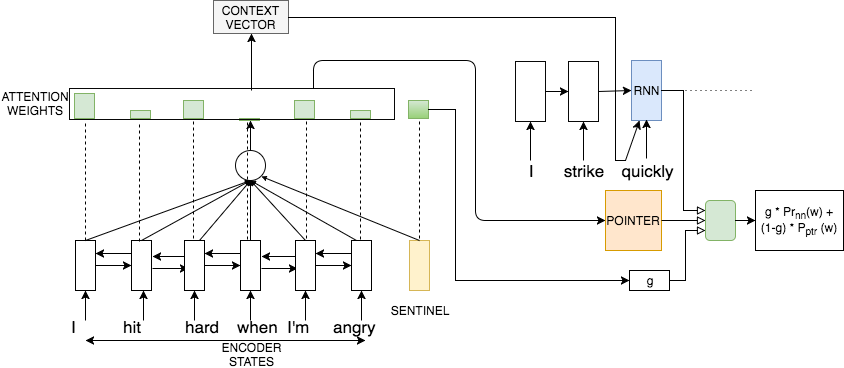
\includegraphics[scale=0.50]{images/StyleTransferGangalVersion.png}
\caption{Pictorial depiction of our overall architecture at decoder step 3. Attention weights are computed using previous decoder hidden state $h_2$, encoder representations, and sentinel vector. Attention weights are shared by decoder RNN and pointer models. The final probability distribution over vocabulary comes from both the decoder RNN and the pointer network. Similar formulation is used over all decoder steps }
\label{fig:architecture}
\end{figure*}


Our overall architecture is shown in Figure (\S\ref{fig:architecture}). We use a bidirectional encoder. We compute soft attention over encoder states. Our decoder side model is a mixture model of RNN module amd pointer network module. The two individual modules share the attentions weights, although it is not necessary to do so. The decoder RNN predicts probability distribution of next word over the vocabulary, while pointer model predicts probability distribution over words in input. The two probabilities undergo a weighted addition, the weights themselves computed based on previous decoder hidden state and the encoder outputs. 

% S2S (sequence-to-sequence) models with attention \cite{bahdanau2014neural} have been used for a variety of tasks like Machine Translation TODO cite. 

Let $\mathbf{x}, \mathbf{y}$ be the some input - output pair in the dataset. Both input $\mathbf{x}$ as well as output $\mathbf{y}$ are sequence of tokens. $\mathbf{x} = \mathbf{x}_1 \mathbf{x}_2 ... \mathbf{x}_{T_{enc}}$, where $T_{enc}$ represents the length of the input sequence $\mathbf{x}$. Similarly, $\mathbf{y} = \mathbf{y}_1 \mathbf{y}_2 ... \mathbf{y}_{T_{dec}} $. Each of $\mathbf{x}_i $, $\mathbf{y}_j $ is be a token from the vocabulary.

\section{Token embeddings} \label{sec:Method2}
Let vocabulary $V$ be the union of modern English and Shakepearean vocabularies i.e. $V = V_{shakespeare} \cup V_{modern}$. Each token is represented by a $M$ dimensional embedding vector. $E_{enc}$ and $E_{dec}$ represent the embedding matrices used by encoder and decoder respectively ( $  E_{enc}, E_{dec} \in \mathbb{R}^{|V| \times M}  $ ). We consider union of the vocabularies for both input and output embeddings because many of the tokens are common in two vocabularies, and in the best performing setting we share embeddings between encoder and decoder models.
Let $E_{enc}(t)$, represent encoder side embeddings of some token $t$. For some input sequence $\mathbf{x}$, $E_{enc}(\mathbf{x})$ is given as $( E_{enc}(\mathbf{x}_1), E_{enc}(\mathbf{x}_2), ... ) $.

\subsection{Pretraining of embeddings}
Considering that we have limited amount of parallel data, learning embeddings in an end-to-end fashion along with the model greatly increases the number of parameters, and is hence not a very good idea.

We pretrain our embeddings on all training sentences. We also experiment with adding additional data from PTB \cite{marcus1993building} for better learning of embeddings. We use the preprocessed PTB data from \cite{mikolov2010recurrent}, which is a standard dataset used in language modelling.

We use the python gensim \footnote{\url{radimrehurek.com/gensim/}} toolkit's implementation of word2vec to train our embeddings. We use four distinct strategies to train our data. In the case where we use external data, we first train the embeddings using both the external data and training data, and then for the same number of iterations on training data alone, to ensure adaptation. Note that we cannot directly use off-the-shelf pre-trained embeddings such as \textit{Glove} \cite{pennington2014glove} and \textit{Word2Vec} \cite{mikolov2013efficient} since we need to learn embeddings for novel word forms (and also different word senses for extant word forms) on the \textit{Original} side.

\subsubsection{Plain}
This method is the simplest pre-training method. Here, we do not use any additional data, and train word embeddings on the union of \textit{Modern} and \textit{Original} sentences. 

\subsubsection{PlainExt}
In this method, we add all the sentences from the external data (\textit{PTB}) to training sentences, and train an embedding on this joint dataset.

\subsubsection{Retro}
\cite{xu2012paraphrasing,xu2014data} also provide a small dictionary $L$ of approximate \textit{Original} $\rightarrow$ \textit{Modern} word pairs, crawled from \url{shakespeare-words.com}, a source distinct from Sparknotes. Since the two \textit{2nd persons} and their corresponding forms (thy, thou, thyself etc) are very frequent but not present in $L$, we add these 4 pairs. Otherwise, we use $L$ as it is. The final dictionary we use has 1524 pairs. \cite{faruqui2014retrofitting} proposed \emph{retrofitting}, a  method to update a learnt set of word embeddings to incorporate pairwise constraints. Given a learnt set of embeddings $p_i \in P$, a vocabulary $V$, and a set $C$ of pairwise constraints $(i,j)$ between words, retrofitting tries to learn a new set of embeddings $q_i \in Q$ to minimize the following objective:
\begin{align*}
    f(Q) & = \delta \sum_{i=1}^{i=|V|} {(p_i-q_i)}^2 + \omega \sum_{(i,j) \in C} {(q_i-q_j)}^2
\end{align*}
We use their off-the-shelf 
implementation \footnote{\url{github.com/mfaruqui/retrofitting}} to encode the dictionary constraints into our pretrained embeddings, setting $C=L$ and using suggested default hyperparameters for $\delta$, $\omega$ and number of iterations.

\subsubsection{RetroExt}
This method is similar to \emph{Retro}, except that we use sentences from the external data (\textit{PTB}) in addition to training sentences.

\subsubsection{None}
Indicates no pretraining.
%\subsubsection{METRO}
%\subsubsection{METROEXT}


%Also, we are hampered by the lack of a standard monolingual dataset for Shakespearean English.

\subsection{\emph{Fixed} embeddings}
Fine-tuning pre-trained embeddings for a given task may lead to \emph{overfitting}, especially in case of small amount of supervised data for the task \cite{madhyastha2015mapping}. This is because embeddings for only a fraction of vocabulary items get updated,  while it doesnt get updated for many vocabulary items. To avoid this, we consider fixed embeddings pretrained as per procedures described earlier. While reporting  results  in Section (\S \ref{sec:Results}), we separately report results for fixed (\emph{FIXED}) and trainable (\emph{VAR}) embeddings, and show that keeping embeddings fixed leads to better performance. 

\section{Method Description} \label{sec:Method3}
In this section we give details of the various modules in the proposed neural model. 

\subsection{Encoder model}
 Let $\overrightarrow{LSTM_{enc}}$ and $\overleftarrow{LSTM_{enc}}$ represent the forward and reverse encoder. $\mathbf{h}^{\overrightarrow{enc}}_{t}$ represent hidden state of encoder model at step $t$ ($\mathbf{h}^{\overrightarrow{enc}}_{t} \in \mathbb{R}^{H} $).
% , the input sequence $\bm{x}$ is of length $I$ and the output sequence $\bm{y}$ is of length $|O|$.
The following equations describe the model:
\begin{center}
\footnotesize
\begin{align*}
    \mathbf{h}^{\overrightarrow{enc}}_0 &=\overrightarrow{0},  \mathbf{h}^{\overleftarrow{enc}}_{|x|} = \overrightarrow{0} \\
    \mathbf{h}^{\overrightarrow{enc}}_{t} &= \overrightarrow{LSTM_{enc}}(\mathbf{h}^{enc}_{t-1},{E_{enc}}({\mathbf{x}_{t}})) \\
    \mathbf{h}^{\overleftarrow{enc}}_{t} &= \overleftarrow{LSTM_{enc}}(\mathbf{h}^{enc}_{t+1},{E_{enc}}({x_{t}})) \\
    \mathbf{h}^{enc}_{t} &= \mathbf{h}^{\overrightarrow{enc}}_{t} + \mathbf{h}^{\overleftarrow{enc}}_{t} 
\end{align*}
\normalsize
\end{center}
We use addition to combine the forward and backward encoder states, rather than concatenation which is standardly used, since it doesn't add extra parameters, which is important in a low-data scenario such as ours. 

%\subsection{Decoder RNN}

\subsection{Attention}

Let $\mathbf{h}_t^{dec}$ represent the hidden state of the decoder LSTM at step $t$. Let $E_{dec}(\mathbf{y}_{t-1})$ represent the decoder side embeddings of previous step output. We use special $START$ symbol at $t=1$. 

We first compute a query vector, which is a linear tranformation of $\mathbf{h}_{t-1}^{dec}$. A sentinel vector $\mathbf{s} \in \mathbb{R}^H$ is concatenated with the encoder states to create $F_{att} \in \mathbb{R} ^ { (T_{enc}+1) \times H } $, where $T_{enc}$ represents the number of tokens in encoder input sequence $\mathbf{x}$. A normalized attention weight vector is computed. The value $g$, which corresponds to attention weight over sentinel vector, represents the weight given to the decoder RNN module while computing output probabilties.
\begin{center}
\footnotesize
\begin{align*}
  \mathbf{q} &= \mathbf{h}_{t-1}^{dec} \,W_{q}   &&  W_{q} \in \mathbb{R}^{H \times H} \\
  F_{att} &= concat( \mathbf{h}^{enc}_{1..T_{enc}}, \mathbf{s} )   && F_{att} \in \mathbb{R}^{(T_{enc}+1) \times H} \\
  \boldsymbol{\alpha}_i &= \sum_{j=1}^{H}( tanh(F_{att}^{(ij)} \, \mathbf{q}_j) ) + \mathbf{b}_i   && \boldsymbol{\alpha}_i, \mathbf{b}_i \in \mathbb{R} \\
  \boldsymbol{\alpha}^{norm} &= softmax(\boldsymbol{\alpha}) && \boldsymbol{\alpha}^{norm} \in \mathbb{R}^{T_{enc}+1} \\
  \boldsymbol{\beta} &= \boldsymbol{\alpha}^{norm}_{1,2,...,T_{enc}} && \boldsymbol{\beta} \in \mathbb{R}^{T_{enc}} \\
  g &= \boldsymbol{\alpha}^{norm}_{T_{enc}+1} && g \in \mathbb{R}
\end{align*}
\normalsize
\end{center}

%  F \,&= \,\text{relu}\, ( I_{proj} \,\oplus\, \mathbf{d}_{proj} ) && F \in \mathbb{R}^{(L+1) \times Q}


\subsection{Pointer model}

%Pointer network
%- motivation: how copy is needed for our task
As noted in (\S \ref{sec:Dataset}), \textit{Original} and \textit{Modern} have significant vocabulary overlap. Moreover, there are lot of proper nouns and rare words which might not be predicted by a sequence to sequence model. To rectify this, pointer networks have been used to enable copying of tokens from input directly \cite{merity2016pointer}. The pointer module provides location based attention, and output probability distribution due to pointer network module can be expressed as follows:
\begin{center}
\footnotesize
\begin{align*}
P_{t}^{PTR}(w) &= \sum_{\mathbf{x}_j=w}( \boldsymbol{\beta}_j )
\end{align*}
\normalsize
\end{center}

\subsection{Decoder RNN}

Output probabilities over vocabulary as per the decoder LSTM module are computed as follows:

% &&  \mathbf{c}_t \in \mathbb{R}^{(L+1) \times Q}
\begin{center}
\footnotesize
\begin{align*}
\mathbf{c}_t &= \sum_{i=1}^{T_{enc}} \boldsymbol{\beta}_i \, \mathbf{h}^{enc}_i  \\
\mathbf{h}^{dec}_{t} &= LSTM(\mathbf{h}^{dec}_{t-1},[\text{concat}({E_{dec}}({\mathbf{y}_{t-1}}),\mathbf{c}_{t})])  \\
P_{t}^{LSTM} &=\text{softmax}(W_{out}[\text{concat}(\mathbf{h}^{dec}_{t}, \mathbf{c}_{t})] + \mathbf{b}^{out}) 
\end{align*}
\normalsize
\end{center}
During training, we feed the ground truth for $\mathbf{y}_{t-1}$, whereas while making predictions on test data, predicted output from previous step is used instead.

\subsection{Output prediction}
As mentioned earlier, final output is a mixture of weighted probabilities from decoder LSTM model and pointer model.  Specifically, output probability of a token $w$ at step $t$ is given as follows:
\begin{center}
\footnotesize
\begin{align*}
P_{t}(w) &= g \times P_{t}^{LSTM}(w) + (1-g) \times P_{t}^{PTR}(w) 
\end{align*}
\normalsize
\end{center}
$P_{t}^{PTR}(w)$ takes a non-zero value only if $w$ occurs in input sequence, otherwise it is $0$.

Setting $g=0$ corresponds to not having a \textit{Copy} component, reducing the model to a plain attentional S2S model, which we refer to as a \textit{SimpleS2S} model. 
%
%
%How are we saving parameters? (expand later)
%\begin{itemize}
%    \item Encoder-decoder embedding sharing
%    \item Pointer-Generation (attention weight) sharing
%    \item Freezing the embeddings 
%\end{itemize}
%
%How are we making learning easier (good starting point)
%\begin{itemize}
%    \item Pretraining embeddings
%    \item Incorporating external dictionary constraints by retrofitting
%    \item Pretraining embeddings on additional monolingual data
%    \item Simple loss function (no auxiliary terms like sentinel loss)
%\end{itemize}
%


\section{Loss functions} \label{sec:Method4}
%Let $i^{th}$ point in dataset be represented by $(\mathbf{x}^{(i)}, \mathbf{y}^{(i)} )$. Let the prediction by model be $\mathbf{y}$

Cross entropy loss is used to train the model.
For a data point $( \mathbf{x}, \mathbf{y} ) \in \mathcal{D}$ and predicted probability distributions $P_t\,(w)$ over the different words $w \in \mathbf{V}$ for each time step $t \in \{1,\ldots,T_{dec}\}$, the loss is given by
\begin{center}
\small
\begin{align*}
  - \sum_{t=1}^{T_{dec}} \,\log p\,\bigl(P_t\,(\mathbf{y}_t) \bigr)
\end{align*}
\normalsize
\end{center}

\subsection{Sentinel Loss (\textsc{SL})}
Following from work by \cite{merity2016pointer}, we consider additional sentinel loss. This loss function can be considered as a form of \emph{supervised attention}. Sentinel loss is given as follows:
\begin{center}
\small
\begin{align*}
  - \sum_{t=1}^{T_{dec}} \,\log ( g^{(t)} + \sum_{x_j=y_t}( \beta^{(t)}_j ) )
\normalsize
\end{align*}
\end{center}


We report the results demonstrating the impact of including the sentinel loss function (\textsc{+SL}).


%\subsection{Initial state of LSTM}
%
%The initial hidden state $h_0$ and initial memory cell state $c_0$ of the LSTM are derived from a transformed combination of the abstract image features produced by the convolutional network, and the input demand embedding.
%For this, we use late fusion on projections of the abstract image features and the demand embedding. The choice of late fusion was driven by the fact that the dimensionality \,($L \times Q$) \,of the image features is much larger than that of the demand embedding. Thus, early fusion may results in the domination of the demand features by the image features.
%
%Let $E_D$ represent embeddings of demand word $D$, and $H$ be the hidden state size of the LSTM network.
%Mathematically, given image features $I_{feats}^{(1)}, \ldots, I_{feats}^{(L)} $ of image $I$, and demand $D$,
%\begin{align}
%  \mathbf{i}_{init} \,&= \,\frac{1}{L} \,\sum_{j=1}^L \Bigl( I_{feats}^{(j)} W_{ih} \Bigr) + \mathbf{b}_{ih} && W_{ih} \in \mathbb{R}^{Q \times (H-M)} \,~\,\text{and} \,~\,\mathbf{b}_{ih} \in \mathbb{R}^{H-M} \\[0.2em]
%  \mathbf{d}_{init} \,&= \,E_d \,W_{dh} + \mathbf{b}_{dh} && W_{dh} \in \mathbb{R}^{M \times M} \,~\,\text{and} \,~\,\mathbf{b}_{dh} \in \mathbb{R}^{M} \\[0.5em]
%  \mathbf{h}_0 \,&= \,\text{tanh}\,(\mathbf{i}_{init}) \,\oplus \,\text{tanh}\,(\mathbf{d}_{init})
%\end{align}
\section{Experiments} \label{sec:Experiments}
\subsection{Preprocessing}
We lowercase sentences and then use NLTK's PUNKT tokenizer to tokenize all sentences. The \textit{Original} side has certain characters like \ae which are not extant in today's language. We map these characters to the closest equivalent character(s) used today (e.g \ae $\rightarrow$ ae)

\subsection{Baseline Methods}
\subsubsection{As-it-is}
Since both source and target side are English, just replicating the input on the target side is a valid and competitive baseline, with a BLEU of $21+$.

\subsubsection{Dictionary}
\cite{xu2012paraphrasing} also use an external, unsupervised dictionary from an external source, which is shared with the dataset. We augment this dictionary with pairs corresponding to the $2$nd person thou (\textit{thou}, \textit{thy}, \textit{thyself}) since these are amongst the most common tokens in the training set.

Directly using this dictionary to perform word-by-word replacement is another admittable baseline. As was noted in the original paper,  this baseline actually performs worse than \textit{As-it-is}. This could be due to its performing aggressive replacement without regard for word context. Moreover, a dictionary cannot easily capture one-to-many mappings as well as long-range dependencies \footnote{thou-thyself and you-yourself}.

\subsubsection{Off-the-shelf SMT}
To train statistical machine translation (\textit{SMT}) baselines, we use the publically available open-source toolkit MOSES \cite{koehn2007moses}, along with the GIZA++  word aligner \cite{och2003minimum}, as was done in \cite{xu2012paraphrasing}. For training the target-side LM component, we use the \textit{lmplz} toolkit within MOSES to train a 4-gram LM. We also use \textit{MERT}  \cite{och2003minimum}, available as part of MOSES, to tune on the validation set.

For fairness of comparison, it is necessary to use the pairwise dictionary and \textit{PTB} while training the SMT models as well. Although SMT does not have mechanisms directly comparable to neural models for incorporating these, the most obvious ways are to use the  dictionary and \textit{PTB} as additional training data for the alignment component and the target-side LM respectively. We experiment with several SMT models, ablating for the use of both \textit{PTB} and dictionary. In \ref{sec:Results}, we only report the performance of the best of these approaches, which uses a 4-gram target-side LM (trained without \textit{PTB}) and an alignment model trained with additional dictionary pairs. The Appendix reports performance for all the approaches.

%We report results with trigram and 4-gram LMs. The LMs are trained using the SRILM toolkit \cite{stolcke2002srilm} available in MOSES. 

\subsection{Evaluation}
Our primary evaluation metric is \emph{BLEU} \cite{papineni2002bleu} . As is standard in the MT community, we compute \emph{BLEU} using the freely available perl script\footnote{\url{http://tinyurl.com/yben45gm}} from the MOSES decoder.

We also use \emph{PINC} \cite{chen2011collecting} as an auxiliary evaluation metric. This metric originates from paraphrase evaluation literature and evaluates how much the target side paraphrases resemble the source side. Given a source sentence $s$ and a target side paraphrase $c$ generated by the system, \emph{PINC(s,c)} is defined as
\begin{center}
\scriptsize
\begin{align*}
    PINC(s,c)&=1-\frac{1}{N} \sum_{n=1}^{n=N} \frac{|Ngram(c,n) \cap Ngram(s,n)|}{|Ngram(c,n)|}
\end{align*}
\normalsize
\end{center}
where $Ngram(x,n)$ denotes the set of n-grams of length $n$ in sentence $x$, and $N$ is the maximum length of ngram considered. We set $N=4$. Higher the \textit{PINC}, greater the novelty of paraphrases generated by the system. Note, however, that PINC does not measure fluency of generated paraphrases.
%\subsection{Pretraining}
%We pretrain our embeddings on all training sentences. We also experiment with adding additional data from PTB \cite{marcus1993building} for better learning of embeddings. We use the preprocessed PTB data from \cite{mikolov2010recurrent}, which is a standard dataset used in language modelling.

%\subsubsection{PLAIN}
%\subsubsection{PLAINEXT}
%\subsubsection{RETRO}
%\cite{xu2012paraphrasing,xu2014data} also provide a small dictionary of approximate Shakespearean English - Modern English word pairs, crawled from \url{shakespeare-words.com}, a source distinct from Sparknotes. Since the two second persons and their corresponding forms (thy, thou, thyself etc) are very frequent but not present in this dictionary, we add these 4 pairs. Otherwise, we use the dictionary as it is. The final dictionary we use has 1524 pairs. \cite{faruqui2014retrofitting} had proposed a  method to update a learnt embedding to incorporate lexicon constraints. We use their off-the-shelf 
%implementation \footnote{\url{https://github.com/mfaruqui/retrofitting}} to incorporate the dictionary constraints into our pretrained embeddings.

%\subsubsection{RETROEXT}

%\subsubsection{METRO}
%\subsubsection{METROEXT}


%We use the python gensim \footnote{\url{https://radimrehurek.com/gensim/}} toolkit's implementation of word2vec to train our embeddings. We use four distinct strategies to train our data.

%In the case where we use external data, we first train the embeddings using both the external data and training data, and then for the same number of iterations on training data alone, to ensure adaptation.

%Note that we cannot directly use off-the-shelf pre-trained embeddings such as \textit{Glove} \cite{pennington2014glove} and \textit{Word2Vec} \cite{mikolov2013efficient} since we need to learn embeddings for novel word forms (and also different word senses for extant word forms) in Early Modern English. %Also, we are hampered by the lack of a standard monolingual dataset for Shakespearean English.

\subsection{Training and Parameters}
We use a minibatch-size of $32$ and the \textit{ADAM} optimizer \cite{kingma2014adam} with learning rate $0.001$,  momentum parameters $0.9$ and $0.999$, and $\epsilon=10^{-8}$. We did not use dropouts for any of our models. All our implementations are coded in Tensorflow 1.1.0 and run on a NVIDIA TitanX GPU. Both our encoder and decoder LSTMs are one layer deep. We do not use multi-layer/stacked LSTMs \cite{luong2015effective} given the paucity of parallel training data.


For every model, we experiment with two configurations of embedding and LSTM size - $S$ (128-128), $M$ (192-192) and $L$ (256-256). Across models, we find that the $M$ configuration performs better in terms of highest validation BLEU.  We also find that larger configurations (384-384 \& 512-512) fail to converge or perform very poorly \footnote{This is expected given the small parallel data}. Here, we report results only for the $M$ configuration for all the models.


\subsection{Validation and Tuning}
For all our models, we pick the best saved model over 15 epochs which has the highest validation BLEU. %For models with SL, $\lambda=0.0025$ is found to work well based on validation set.

\subsection{Decoding}
At test-time we use greedy decoding to find the most likely target sentence\footnote{Empirically, we observed that beam search does not give improvements for our task}. We also experiment with a post-processing strategy which replaces \emph{UNKs} in the target output with the highest aligned (maximum attention) source word. We find that this gives a small jump in \emph{BLEU} of about 0.1-0.2 for all neural models \footnote{Since effect is small and uniform, we report BLEU before post-processing in Table \ref{tab:knightExp} }. Our best model, for instance, gets a jump of 0.14 to reach a BLEU of \emph{\textbf{31.26}} from 31.12.




\section{Results} \label{sec:Results}

\begin{figure}
\captionsetup[subfigure]{labelformat=empty}
\captionsetup[subfigure]{justification=centering}
\begin{subfigure}{0.2\textwidth}
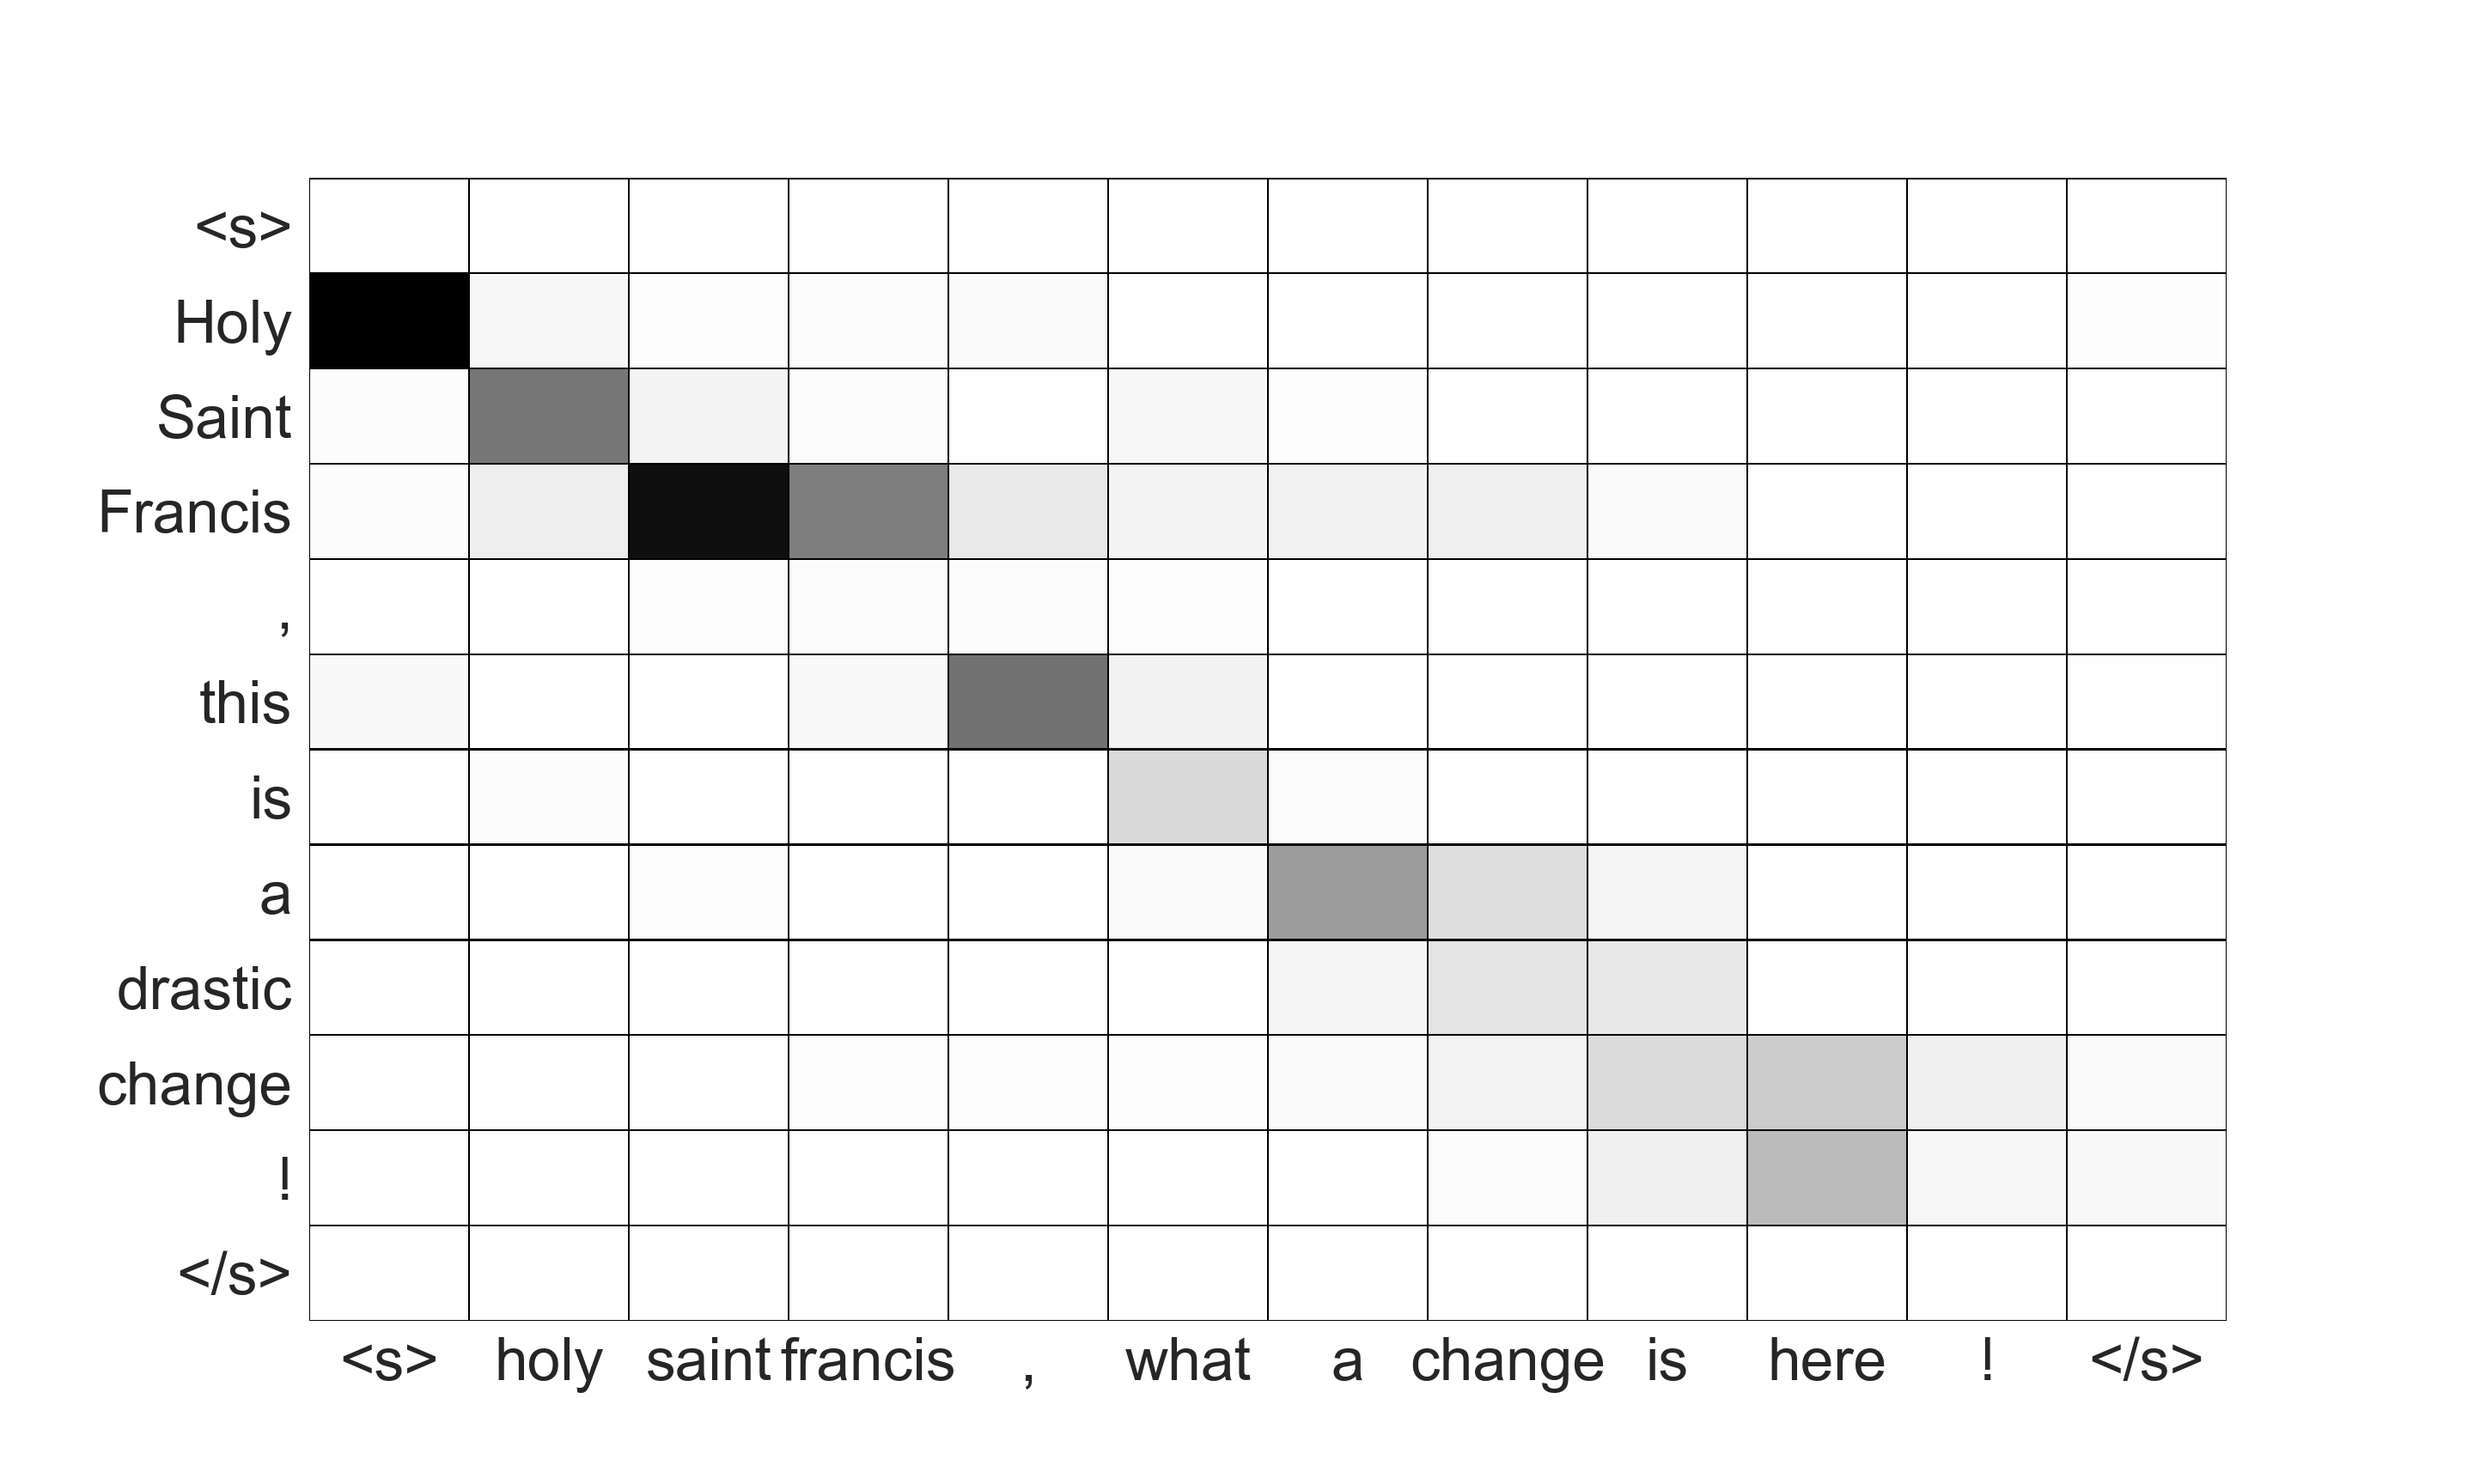
\includegraphics[scale=0.20]{HolySaintFrancisCopy.png}
%\captionsetup{format=hang}
%\caption{Copy Model}
%\label{fig:attention}
\end{subfigure} \hspace{0.15\textwidth}
\begin{subfigure}{0.2\textwidth}
\centering
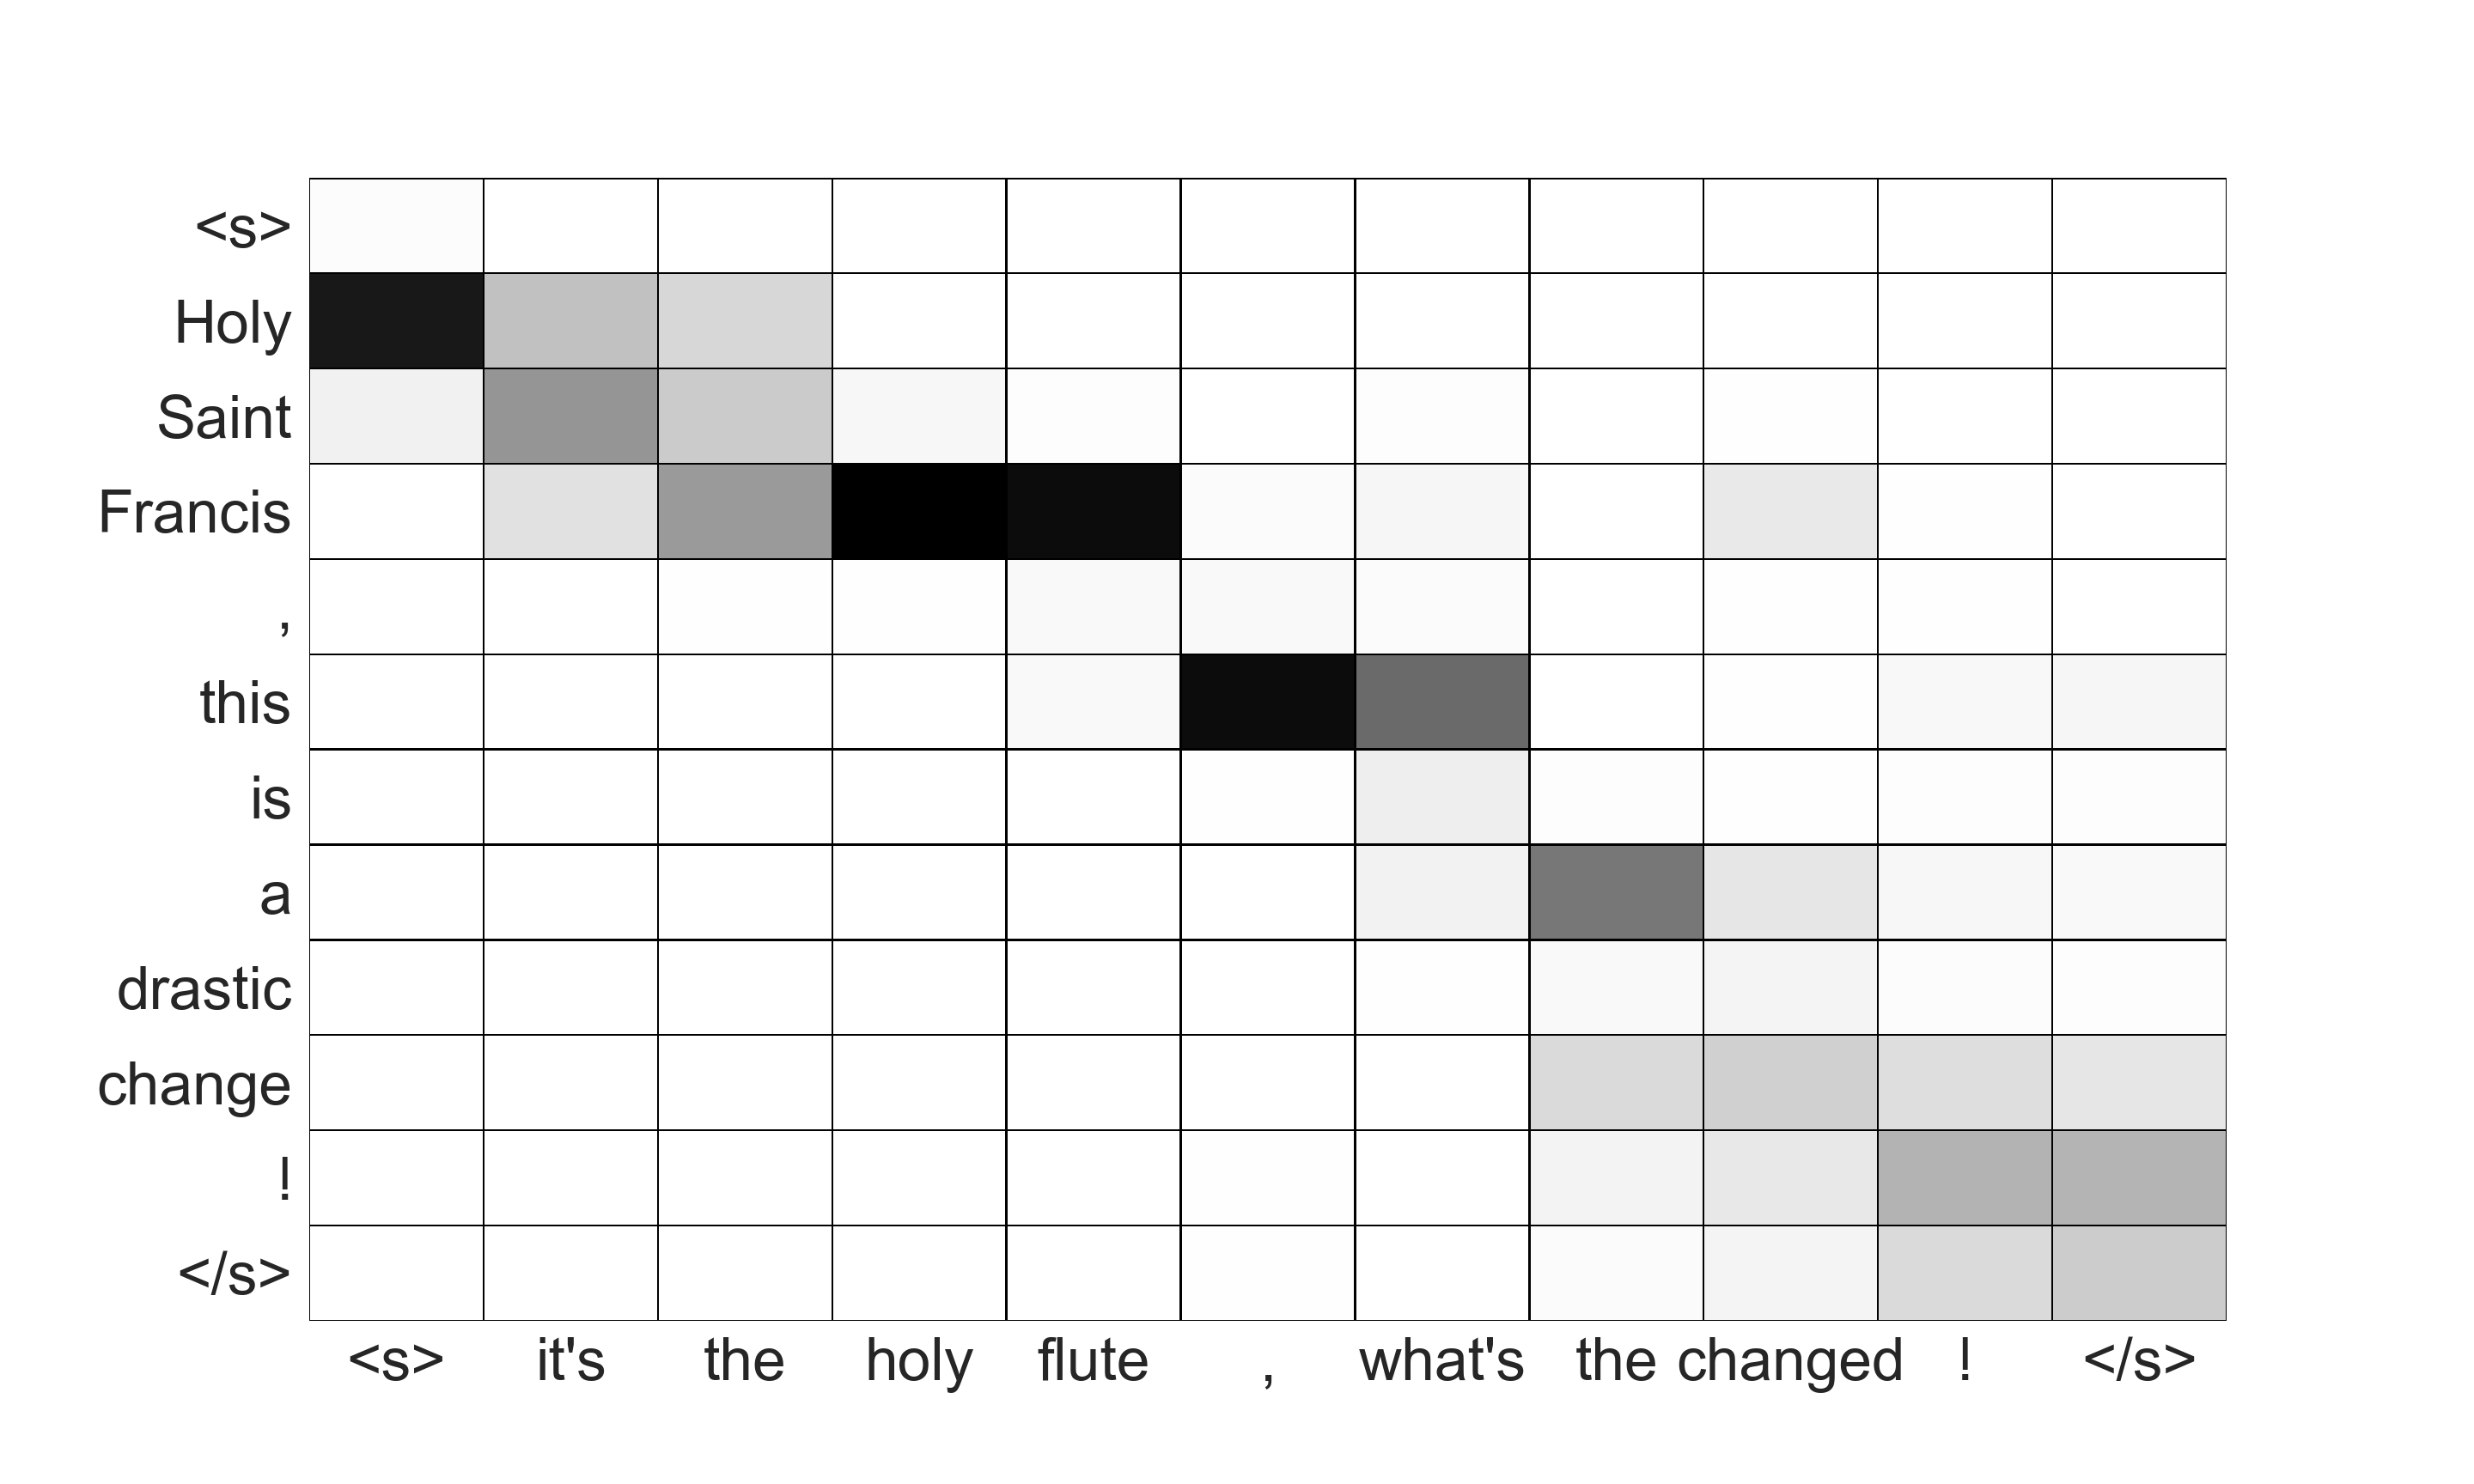
\includegraphics[scale=0.20]{HolySaintFrancisS2S.png}
%\caption{}
%\label{fig:attention2}
\end{subfigure}
\caption{Attention matrices from a \emph{Copy} (top) and a \textit{simple S2S} (bottom) model respectively on the input sentence \textit{``Holy Saint Francis, this is a drastic change!"} . \textbf{$<s>$} and \textbf{$</s>$} are  start and stop characters. Darker cells are higher-valued.}
\textbf{\label{fig:attention}}
\end{figure}

%- BLEU and other measures
%
%- baseline
%- rnn soft attention
%- pointer copy
%- sentinel loss


%Pretrained embeddings
%- different versions
%- trainable vs. non trainable


%Qualitative results
%- good examples, bad examples
%- examples demonstrating copy
The results in Table \ref{tab:knightExp} confirm most of our hypotheses about the right architecture for this task.
\begin{itemize}
    \item \textbf{Copy component}: We can observe from Table \ref{tab:knightExp} that the various \emph{Copy} models each outperform their \emph{SimpleS2S} counterparts by atleast 7-8 BLEU points.
    \item \textbf{Retrofitting dictionary constraints}: The \emph{Retro} configurations generally outperform their corresponding \emph{Plain} configurations. For instance, our best configuration \emph{Copy.Yes.RetroExtFixed} gets a better BLEU than \emph{Copy.Yes.PlainExtFixed} by a margin of atleast 11.
    \item \textbf{Sharing Embeddings}: Sharing source and target side embeddings benefits all the \emph{Retro} configurations, although it slightly deteriorates performance (about 1 BLEU point) for some of the \emph{Plain} configurations. 
    \item \textbf{Fixing Embeddings}: \emph{Fixed} configurations always perform better than corresponding \emph{Var} ones (save some exceptions). For instance, \emph{Copy.Yes.RetroExtFixed} get a BLEU of 31.12 compared to 20.95 for \emph{Copy.Yes.RetroExtVar}. Due to fixing embeddings, the former has just half as many parameters as the latter (5.25M vs 9.40M)
    \item \textbf{Effect of External Data}: Pretraining with external data \emph{Ext} works well along with retrofitting \emph{Retro}. For instance, \emph{Copy.Yes.RetroExtFixed} gets a BLEU improvement of 2+ points over \emph{Copy.Yes.RetroFixed}
    \item \textbf{Effect of Pretraining}: For the \emph{SimpleS2S} models, pre-training adversely affects BLEU. However, for the \emph{Copy} models, pre-training leads to improvement in BLEU. The simplest pretrained \emph{Copy} model, \emph{Copy.No.PlainVar} has a BLEU score 1.8 higher than \emph{Copy.No.NoneVar}.
    \item \textbf{PINC scores}: All the neural models have higher PINC scores than the statistical and dictionary approaches, which indicate that the target sentences produced differ more from the source sentences than those produced by these approaches.
    \item \textbf{Sentinel Loss:} Adding the sentinel loss does not have any significant effect, and ends up reducing BLEU by a point or two, as seen with the \emph{Copy+SL} configurations.
\end{itemize}

\subsection{Qualitative Analysis}
Figure \ref{fig:attention} shows the attention matrices from our best \textit{Copy} model (\emph{Copy.Yes.RetroExtFixed}) and our best \textit{SimpleS2S} model (\emph{SimpleS2S.Yes.Retrofixed}) respectively for the same input test sentence. Without an explicit \textit{Copy} component, the \textit{SimpleS2S} model cannot predict the words \textit{saint} and \textit{francis}, and drifts off after predicting incorrect word \textit{flute}.

Table \ref{tab:intro} presents model outputs\footnote{All neural outputs are lowercase due to our preprocessing. Although this slightly affects BLEU, it helps prevent token occurrences getting split due to capitalization.} for some test examples. In general, the \textit{Copy} model outputs resemble the ground truth more closely compared to \textit{SimpleS2S} and \textit{Stat} . In some cases, it faces issues with repetition (Examples 5 and 7) and fluency (Example 9).


\section{Related Work} \label{sec:RelatedWord}

%style adaptation
There have been some prior work on style adaptation. Xu et al. \shortcite{xu2012paraphrasing} use phrase table based statistical machine translation to transform text to target style.  % \cite{xu2014data}
On the other hand our method is an end-to-end trainable neural network.
Saha Roy et al \shortcite{saha2015automated} leverage different language models based geolocation and occupation to align a text to specific style. However, their work is limited to addition of adjectives and adverbs. Our method can handle more generic tranformations including addition and deletion of words.

S2S neural models were first proposed by \cite{sutskever2014sequence}. Furthermore, \cite{bahdanau2014neural} enriched these methods with a attention mechanism , giving state-of-the-art results for MT. Since then, these models have been applied to many tasks like parsing \cite{vinyals2015pointer} and summarization \cite{rush2015neural}. In the context of MT, various settings such as multi-source MT \cite{zoph2016multi}, many-to-many MT \cite{johnson2016google}, MT with external information \cite{sennrich2016controlling} have been explored. Distinct from all of these, our work attempts to solve a Modern $\rightarrow$ Original English style transfer task. Although our task is closely related to both paraphrasing and MT, it has some unique task-specific properties such as considerable source-target overlap in vocabulary and grammar (unlike MT), while at the same time not sharing the source and target language (unlike paraphrasing). Unlike text simplification and summarization, our task does not involve shortening content length. 

Pointer networks \cite{vinyals2015pointer} allow the use of input-side words directly as output in a neural S2S model, and have been used for tasks like extractive summarization \cite{see2017get} \cite{zeng2016efficient}  and question answering \cite{wang2016machine}. However, pointer networks cannot generate words not present in the input. A mixture model of recurrent neural network and pointer network has been shown to achieve good performance on language modeling task \cite{merity2016pointer}. Gu et al \shortcite{gu2016incorporating} also proposed a mixture model pointer network - \textit{COPYNET} for sequence to sequence tasks. A major motivation for the development of pointer networks was their ability to easily copy tokens corresponding to rare words, proper nouns and entity names from the input-side. Distinct from the prior work on such networks, the high source-target language overlap for our task provides an added motivation to use them, and our experiments illustrate this utility.


\section{Conclusion} \label{sec:Conclusion}
We demonstrate automatic approaches to transform Modern English text to Shakespearean English. Our work provides insights on the utility of incorporating input-copying, embedding sharing and dictionary constraints for problems with shared (but non-identical) source-target sides and sparse parallel data. We also release our code for further research on this and related tasks\footnote{Linked to in supp.material to preserve anonymity}.

Sparknotes also provides similar translations to Modern English for \textit{Beowulf} \footnote{\url{tinyurl.com/d5ntme7}} (Old English) and \textit{Canterbury Tales}  (Middle English).  A point of future work would be develop similar models to translate to these styles/languages. An additional extension would be to develop a single encoder-decoder model for translation to any diachronic English style, in the manner of \cite{johnson2016google}.

%\footnote{\url{http://tinyurl.com/ya9sd4k}}

\begin{table}
\centering
\scriptsize
%\begin{center}
%\scriptsize
\addtolength{\tabcolsep}{-2pt}
\begin{tabular}{|l|l|l|l| }
\hline 
Model & Sh  & Init  & BLEU (PINC) \\ \hline \hline
\textsc{As-it-is}  & {-} & {-}  &  {21.13} (0.0)  \\ \hline
\textsc{Dictionary}  & {-} & {-}  &  {17.00} (26.64)  \\ \hline
%\textsc{GIZA++} (3LM)  & {-} & {-}  &  {22.26} (28.34)  \\ \hline
%\textsc{GIZA++} (4LM)  & {-} & {-}  &  {24.17} (28.14)   \\ \hline
%\textsc{GIZA++} (4LM.3)  & {-} & {-}  &  {24.10} (25.86)   \\ \hline
%\textsc{GIZA++} (4LM.4)  & {-} & {-}  &  {23.76} (25.86)   \\ \hline
%\textsc{GIZA++} (4LM.5)  & {-} & {-}  &  {23.87} (21.85)   \\ \hline
%\textsc{GIZA++} (4LM.6)  & {-} & {-}  &  {23.81} (23.60)    \\ \hline
\textsc{Stat}   & {-} & {-}  &  \textbf{24.39} (32.30)    \\ \hline
%\textsc{GIZA++} (4LM.8)  & {-} & {-}  &  {24.21} (30.05)    \\ \hline
%\textsc{GIZA++} (4LM.9)  & {-} & {-}  &  {23.73} (23.48)   \\ \hline
\multirow{10}{*}{\textsc{SimpleS2S}} &  $\times$ & $NoneVar$ & 11.66 (85.61) \\
%$\times$ & $NONEVAR$ & 9.33 \\
%&  $\times$ & $PLAINVAR$ & 8.73 \\
&  $\times$ & $PlainVar$ & 9.27 (86.52) \\
 & $\times$ & $PlainExtVar$  & 8.73 (87.17) \\ 
 & $\times$ & $RetroVar$ &  10.57 (85.06) \\ 
 %& $\times$ & $RETROEXTVAR$  & 10.05 \\
& $\times$ & $RetroExtVar$  & 10.26 (83.83) \\ 
% & $\checkmark$ & $NONEVAR$ &  10.51 \\
& $\checkmark$ & $NoneVar$ &  11.17 (84.91) \\
% & $\checkmark$ & $PLAINVAR$ &  8.82 \\
 & $\checkmark$ & $PlainVar$ &  8.78 (85.57) \\
% & $\checkmark$ & $PLAINFIXED$ &  8.83\\
 & $\checkmark$ & $PlainFixed$ &  8.73 (89.19)\\
 %& $\checkmark$ & $PLAINEXTVAR$  & 9.18 \\
 & $\checkmark$ & $PlainExtVar$  & 8.59 (86.04) \\
 %& $\checkmark$ & $PLAINEXTFIXED$  & 9.20 \\
 & $\checkmark$ & $PlainExtFixed$  & 8.59 (89.16) \\
 %& $\checkmark$ & $RETROVAR$ &  10.56 \\
 & $\checkmark$ & $RetroVar$ &  10.86 (85.58) \\
 %& $\checkmark$ & $RETROFIXED$ &  10.54 \\
 & $\checkmark$ & $RetroFixed$ &  11.36 (85.07) \\
 %& $\checkmark$ & $RETROEXTVAR$  & 9.96 \\
 & $\checkmark$ & $RetroExtVar$  & 11.25 (83.56) \\
 %& $\checkmark$ & $RETROEXTFIXED$  & \textbf{9.96} \\  
 & $\checkmark$ & $RetroExtFixed$  & \textbf{10.86} (88.80) \\  \hline
\multirow{6}{*}{\textsc{Copy}} & $\times$ & $NoneVar$ & 18.44 (83.68) \\
%& $\times$ & $NONEVAR$ & 21.31 \\
% & $\times$ & $PLAINVAR$ & 19.52 \\
 & $\times$ & $PlainVar$ & 20.26 (81.54) \\ %f
 %& $\times$ & $PLAINEXTVAR$  & 18.11 \\ 
 & $\times$ & $PlainExtVar$  & 20.20 (83.38)\\ 
 %& $\times$ & $RETROVAR$ &  21.36 \\
 & $\times$ & $RetroVar$ &  21.25 (81.18) \\
 %& $\times$ & $RETROEXTVAR$  & 20.10 \\
 & $\times$ & $RetroExtVar$  & 21.57 (82.89) \\
 %& $\checkmark$ & $NONEVAR$ &  23.01 \\
  & $\checkmark$ & $NoneVar$ &  22.70 (81.51) \\
 %& $\checkmark$ & $PLAINVAR$ &  20.95 \\ 
 & $\checkmark$ & $PlainVar$ &  19.27 (83.87) \\ 
 %& $\checkmark$ & $PLAINFIXED$ &  23.56 \\
 & $\checkmark$ & $PlainFixed$ &  21.20 (81.61) \\
 %& $\checkmark$ & $PLAINEXTVAR$  & 20.33 \\
 & $\checkmark$ & $PlainExtVar$  & 20.76 (83.17) \\
% & $\checkmark$ & $PLAINEXTFIXED$  & 21.67 \\
 & $\checkmark$ & $PlainExtFixed$  & 19.32 (82.38) \\
 %& $\checkmark$ & $RETROVAR$ &  20.90 \\
 & $\checkmark$ & $RetroVar$ &  22.71 (81.12) \\
% & $\checkmark$ & $RETROFIXED$ &  \textbf{28.80} \\
 & $\checkmark$ & $RetroFixed$ &  \textbf{28.86} (80.53) \\
 %& $\checkmark$ & $RETROEXTVAR$  & 22.61 \\
 & $\checkmark$ & $RetroExtVar$  & 20.95 (81.94) \\
 %& $\checkmark$ & $RETROEXTFIXED$  & \textbf{30.42} (81.13) \\
 %& $\checkmark$ & $RETROEXTFIXED,192$  & \textbf{31.02} (80.62) \\
 %& $\checkmark$ & $RETROEXTFIXED,256$  & \textbf{31.06} (80.69) \\
 & $\checkmark$ & $RetroExtFixed$  & \textbf{31.12} (79.63) \\
 %& $\checkmark$ & $RETROEXTFIXED-L,128$  & \textbf{27.86} (0.0) \\
 %& $\checkmark$ & $RETROEXTFIXED-L,192$  & \textbf{28.38} (0.0) \\
 %& $\checkmark$ & $RETROEXTFIXED-L,256$  & \textbf{29.37} (0.0) \\
 \hline
\multirow{6}{*}{\textsc{Copy+SL}} & $\times$ & $NoneVar$ & 17.88 (83.70) \\
& $\times$ & $PlainVar$ & 20.22 (81.52) \\
 & $\times$ & $PlainExtVar$  & 20.14 (83.46) \\   
 & $\times$ & $RetroVar$ &  21.30 (81.22) \\ 
 & $\times$ & $RetroExtVar$  & 21.52 (82.86) \\ 
 & $\checkmark$ & $NoneVar$ &  22.72 (81.41) \\
 & $\checkmark$ & $PlainVar$ &  21.46 (81.39) \\ 
 %& $\checkmark$ & $PLAINFIXED$ &  23.76 \\
 & $\checkmark$ & $PlainFixed$ &  23.76 (81.68) \\
 %& $\checkmark$ & $PLAINEXTVAR$  & 0.0 \\
 & $\checkmark$ & $PlainExtVar$  & 20.68 (83.18) \\
 %& $\checkmark$ & $PLAINEXTFIXED$  & 21.59 \\
 & $\checkmark$ & $PlainExtFixed$  & 22.23 (81.71) \\
 & $\checkmark$ & $RetroVar$ &  22.62 (81.15) \\ 
 %& $\checkmark$ & $RETROFIXED$ &  28.60 \\
 & $\checkmark$ & $RetroFixed$ &  27.66 (81.35) \\
 & $\checkmark$ & $RetroExtVar$  & 24.11 (79.92) \\ 
 %& $\checkmark$ & $RETROEXTFIXED,\lambda=2$  & \textbf{11.51} \\ 
 %& $\checkmark$ & $RETROEXTFIXED,\lambda=0.25$  & \textbf{25.54} \\
 %& $\checkmark$ & $RETROEXTFIXED,\lambda=0.025$  & 30.03 \\
 %& $\checkmark$ & $RETROEXTFIXED,\lambda=0.0125$  & 30.12 \\
 %& $\checkmark$ & $RETROEXTFIXED,\lambda=0.0075$  & 0.0 \\
 %& $\checkmark$ & $RETROEXTFIXED$  & 30.34 \\
 & $\checkmark$ & $RetroExtFixed$  & 27.81 (84.67) \\
 %& $\checkmark$ & $RETROEXTFIXED,\lambda=0.0025$  & 30.30 \\
 \hline 
\end{tabular}
%\end{center}
\caption{Test BLEU results. \emph{Sh} denotes encoder-decoder embedding sharing (\textit{No}=$\times$,\textit{Yes}=$\checkmark$) . \emph{Init} denotes the manner of initializing embedding vectors. The \emph{-Fixed} or \emph{-Var} suffix indicates whether embeddings are fixed or trainable. \textsc{COPY} and \textsc{SIMPLES2S} denote presence/absence of \textit{Copy} component. \textsc{+SL} denotes sentinel loss.}
\textbf{\label{tab:knightExp}}
\end{table}

%Training on monolingual corpora in Early Modern English, and also experiment with noisy-channel like neural models \cite{yu2016neural}, which directly factor in a language model like traditional SMT, but with additional benefits of embedding approaches.

%\textit{COPY} and \textit{SIMPLES2S} denote attentional S2S models with/without a copy component respectively, while \textit{+SL} denotes usage of sentinel loss.



%\section*{Acknowledgments}

%Do not number the acknowledgment section.

\bibliography{emnlp2017}
\bibliographystyle{emnlp_natbib}

\end{document}
